\documentclass[11pt]{article}

% use packages
\usepackage[utf8]{inputenc}
\usepackage{amsmath}
\usepackage{amsthm}
\usepackage{amsfonts}
%\usepackage{amscd}
\usepackage{amssymb}
\usepackage{graphicx}
\usepackage{mathtools}
\usepackage{natbib}
\usepackage{enumitem}
\usepackage{url}
\usepackage{authblk}
\usepackage{bm}
\usepackage[usenames]{color}
\usepackage{hyperref}
\usepackage{geometry}
\usepackage{caption}
\usepackage{tikz}
% margin setup
\geometry{margin=1in}


% function definition
\newcommand{\R}{\mathbb{R}}
\newcommand{\w}{\textbf{w}}
\newcommand{\x}{\textbf{x}}
\newcommand{\X}{\textbf{X}}
\newcommand{\Y}{\textbf{Y}}
\newcommand{\Hist}{\mathcal{H}}
\def\mbf#1{\mathbf{#1}} % bold but not italic
\def\ind#1{\mathrm{1}(#1)} % indicator function
\newcommand{\simiid}{\stackrel{iid}{\sim}} % IID 
\def\where{\text{ where }} % where
\newcommand{\indep}{\perp \!\!\! \perp } % independent symbols
\def\cov#1#2{\mathrm{Cov}(#1, #2)} % covariance 
\def\mrm#1{\mathrm{#1}} % remove math
\newcommand{\reals}{\mathbb{R}} % Real number symbol
\def\t#1{\tilde{#1}} % tilde
\def\normal#1#2{\mathcal{N}(#1,#2)} % normal
\def\mbi#1{\boldsymbol{#1}} % Bold and italic (math bold italic)
\def\v#1{\mbi{#1}} % Vector notation
\def\mc#1{\mathcal{#1}} % mathical
\DeclareMathOperator*{\argmax}{arg\,max} % arg max
\DeclareMathOperator*{\argmin}{arg\,min} % arg min
\def\E#1{\mathrm{E}(#1)} % Expectation symbol
\def\var#1{\mathrm{Var}(#1)} % Variance symbol
\def\checkmark{\tikz\fill[scale=0.4](0,.35) -- (.25,0) -- (1,.7) -- (.25,.15) -- cycle;} % checkmark
\newcommand\red[1]{{\color{red}#1}}


\newcommand{\norm}[1]{\left\lVert#1\right\rVert} % A norm with 1 argument
\DeclareMathOperator{\Var}{Var} % Variance symbol

\newtheorem{cor}{Corollary}
\newtheorem{lem}{Lemma}
\newtheorem{thm}{Theorem}
\newtheorem{defn}{Definition}
\newtheorem{prop}{Proposition}
\theoremstyle{definition}
\newtheorem{remark}{Remark}
\hypersetup{
  linkcolor  = blue,
  citecolor  = blue,
  urlcolor   = magenta,
  colorlinks = true,
} % color setup

% proof to proposition 
\newenvironment{proof-of-proposition}[1][{}]{\noindent{\bf
    Proof of Proposition {#1}}
  \hspace*{.5em}}{\qed\bigskip\\}
% general proof of corollary
  \newenvironment{proof-of-corollary}[1][{}]{\noindent{\bf
    Proof of Corollary {#1}}
  \hspace*{.5em}}{\qed\bigskip\\}
% general proof of lemma
  \newenvironment{proof-of-lemma}[1][{}]{\noindent{\bf
    Proof of Lemma {#1}}
  \hspace*{.5em}}{\qed\bigskip\\}

\allowdisplaybreaks



% title
\title{Minimizing post shock forecasting error using disparate information}
\author{Jilei Lin\thanks{jileil2@ilinois.edu}}
\author{Ziyu Liu\thanks{ziyuliu3@illinois.edu}}
\author{Daniel J. Eck\thanks{dje13@illinois.edu}}
\affil{Department of Statistics, University of Illinois at Urbana-Champaign}

%%% New version of \caption puts things in smaller type, single-spaced 
%%% and indents them to set them off more from the text.
\makeatletter
\long\def\@makecaption#1#2{
  \vskip 0.8ex
  \setbox\@tempboxa\hbox{\small {\bf #1:} #2}
  \parindent 1.5em  %% How can we use the global value of this???
  \dimen0=\hsize
  \advance\dimen0 by -3em
  \ifdim \wd\@tempboxa >\dimen0
  \hbox to \hsize{
    \parindent 0em
    \hfil 
    \parbox{\dimen0}{\def\baselinestretch{0.96}\small
      {\bf #1.} #2
      %%\unhbox\@tempboxa
    } 
    \hfil}
  \else \hbox to \hsize{\hfil \box\@tempboxa \hfil}
  \fi
}
\makeatother

\begin{document}

\begin{center}
  \textbf{Note}
\end{center}


Things to do:
\begin{enumerate}
  \item Literature review and introduction (We need a literature review for existing methods that are similar/different but close enough methods.  Possible searches include pooling, time series pooling, bayesian time series, bayesian autoregression)
  \item Explore bootstrapping
  \item Data analysis
\end{enumerate}

In R, \texttt{optim} function in \texttt{base} and \texttt{Rsolnp} package may be helpful for solving the minimization problems in synthetic control methods.


\begin{center}
  \textbf{Updates in this version}
\end{center}

\begin{enumerate}
  \item The manuscript is revised according to the comments and unnecessary parts are deleted.
  \item Parametric bootstrap for AR(1) is added in Section  3.3 with some references added.
  \item A couple of references are added in the introduction but more to be added.
\end{enumerate}


% table of contents
\tableofcontents


\newpage 

\maketitle
\begin{abstract}
    We develop a forecasting methodology for time series data that has 
    undergone a shock. We still can provide credible forecasts for a time 
    series in the presence of such systematic shocks by drawing from disparate 
    time series that have undergone similar shocks for which post-shock 
    outcome data is recorded.  These disparate time series are assumed to have 
    mechanistic similarities to the time series under study but are otherwise 
    independent (Granger noncausal).  The inferential goal of our forecasting 
    methodology is to supplement observed time series data with post-shock 
    data from the disparate time series in order to minimize average forecast 
    risk. 
\end{abstract}




\section{Introduction}
The technique of combining forecasts to lower forecast error has a rich 
history \citep{bates1969combination, mundlak1978pooling, 
  timmermann2006forecast, granger2014forecasting}.  
The Introduction of \citet{timmermann2006forecast} provided several reasons 
for combining forecasts.  In particular, combining forecasts may be 
beneficial when: 
1) the information set underlying individual forecasts is often unobserved to 
the forecast user; 2) different individual forecasts may be very differently 
affected by non-stationarities and model misspecifications; 3) different 
individual forecasts may be motivated by different loss functions 
\citep[and references therein]{timmermann2006forecast}.
The setting for the forecast combination problem is that there are 
competing forecasts for a single time series.  In this setting, one may 
desire combining forecasts as a method for lowering overall forecast error.  




In this article we provide forecasting adjustment techniques with the goal 
of lowering overall forecast error when the time series under study has 
undergone a structural shock.
%In this article we propose a new setting for the forecast combination 
%problem.  We will suppose that a time series of interest has recently 
%undergone a structural shock that is not similar to anything observed in its 
%past, and we desire reliable post-shock forecasts in this setting.  
It is unlikely that any forecast that previously gave successful predictions 
for the time series of interest will be able to accommodate the 
structural shock.  Therefore the traditional forecast combination framework 
may not be of any help. However, all is not lost in this setting. It may be 
the case that there exists disparate time series that have previously 
undergone similar structural shocks.  When this is so, one may be able to 
aggregate the post-shock information from these disparate time series to 
aid the post-shock forecast for the time series under investigation.  

We develop and compare aggregation techniques in this post-shock setting and 
investigate settings for when they do and do not decrease mean squared 
prediction error. We assume a simple auto regressive data generating process 
with a general random effects structure. The main idea is to first average 
the estimated shock effects from the disparate time series and then add 
the averaged estimated shock effect to the present forecast. When these 
time series are independent and the mean of shock effect distribution is 
large relative to its variance then this technique will reduce mean squared 
prediction error under the assumed model. Note that this methodology is not 
motivated with the goal of unbiased, asymptotically unbiased, or consistent 
estimation for the shock-effect of the time series under study. We consider 
three aggregation techniques: simple averaging, inverse-variance weighted 
averaging, and similarity weighting. The latter technique is similar to 
the weighting in synthetic control methodology \citep{abadie2010synthetic}.


\vspace{.3cm}

\emph{\textcolor{red}{More to be added ...}}

\vspace{.3cm}

Time-series pooling methodology is one of the main methods to deal this problem. The literature of time-series pooling is mainly related to pooling cross-sectional data. In this setting, estimation of parameters is usually based on merging from different time series using various pooling techniques.  For example, \citet{zellner1991forecasting} assumes the coefficient vectors of different time series are the same so that the time series can be merged to estimate parameters once in forecasting turning point of GDP growth rate in practice. 

\emph{\textcolor{red}{More to be added ...}}


Modern research in ``combining'' forecasts from disparate time series have taken perspectives from distinct fields.  \citet{lee2020estimation} constructed a Bayesian hierarchical model  to estimate posterior parameters for Richards model to improve predictive precision of COVID-19 infection trajectories for different countries. Though a Bayesian hierarchical approach can be a solution for our problem by setting up prior for shock-effects, the analysis is sensitive to the prior and the hierarchical model setup, and conditions for predictive improvement are generally hard to know. \citet{plessen2020integrated} employs a data-mining approach to take COVID-19 data from different countries as input to predict \emph{global} net daily infections  and deaths of COVID-19 from clustering. However, the fit is poor due to tremendous volatility of COVID-19 data, and perhaps a lack of random structure in his model. 

\emph{\textcolor{red}{More to be added ...}}



\begin{figure}[t]
  \begin{center}
    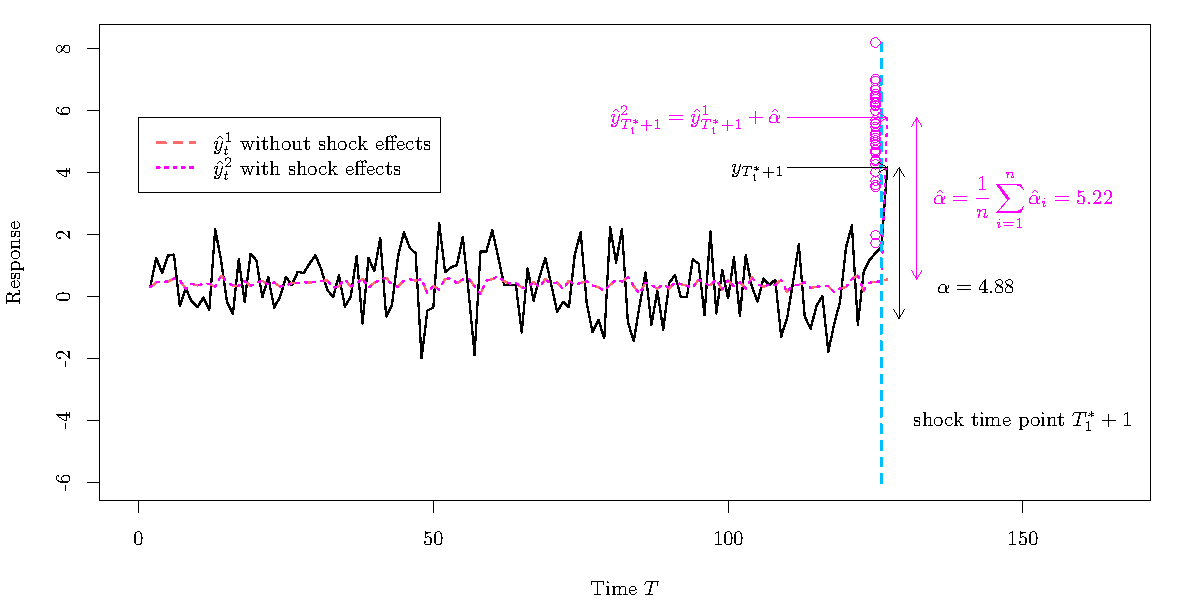
\includegraphics[height = 8cm]{comp.pdf}
    \caption{A comparison between forecast without considering shock effects and the one uses simple averaging given $n=40$ disparate time series and that the shock time is at $T_1^* = 125$.}\label{figure1}
  \end{center}  
  \vspace{-.6cm}
\end{figure}





%The question is then how to estimate the shock effects and improve the 
%prediction? This paper proposes three estimators, the adjustment estimator, weighted adjustment estimator, and inverse-variance weighted estimators. Section (to be updated) discusses properties of those estimators. Section (to be updated) compares the  interplay between prediction risk and different shock effects estimators. Section (to be updated) conducts simulation to justify our claims and certain properties that cannot be found analytically.



\section{Setting}
\label{setting}
We will suppose that an analyst has time series data ($y_{i,t}$,$\x_{i,t}$), 
$t = 1$, $\ldots$, $T_i$, $i = 1$, $\ldots$, $n+1$, where $y_{i,t}$ is a 
scalar response and $\x_{i,t}$ is a vector of covariates that are revealed to 
the analyst prior to the observation of $y_{1,t}$.  Suppose that the analyst 
is interested in forecasting $y_{1,t}$, the first time series in the 
collection.
%$y_1, y_2, \ldots$.  
%Given each time point $t \geq 1$, let $\x_{1,t}$ be a vector of covariates 
%revealed prior to the observation of $y_{1,t}$.  
To gauge the performance of a procedure that produces forecasts 
$\{\hat y_{1,t}, t= 1,2,\ldots\}$ given time horizon $T_1$, we consider the 
average forecast risk
$$
  R_T = \frac{1}{T}\sum_{t=1}^T\E{\hat y_{1,t} - y_{1,t}}^2
$$
in our analyses. In this article, we consider a similar dynamic panel data 
model with autoregressive structure to that in \citet{blundell1998initial}. 
%without past time period covariate 
%information and with a single present time covariate.  
Our dynamic panel model includes an additional shock effect whose presence 
or absence is given by the binary variable $D_{i,t}$, the details of this model 
are in the next section.

Figure \ref{figure1} provides simple intuition of the practical usefulness of our proposed methodology. This figure depicts a time-series that experienced a ``shock'' at time point $T_1^* = 125$. It is supposed that the researcher does not have any information beyond $T_1^*$, but does have observations of forty disparate time series that have previously undergone a similar shock for which post-shock responses are recorded. Similarity in this context means that the shock effects are random variables that from a common distribution.
%As we can see, the purple line provides a better prediction than the red line in this particular example. But we will justify later that consideration of estimated shock-effects will improve the prediction under certain conditions.
In this example, the mean of the estimated shock effects is taken as a shock-effect estimator for the time series under study. Forecasts are then made by adding this shock-effect estimator to the estimated response values obtained from the process that ignores the shock. It is apparent from Figure \ref{figure1} that adjusting forecasts in this manner 1) leads to a reduction in forecasting risk; 2) does not fully recover the true shock-effect. We evaluate the performance of this post-shock prediction methodology throughout this article; we outline situations for when it is expected to work and when it is not.

%Section \ref{properties} will provide a more detailed treatment about when our proposed estimators in Section \ref{constructionofestimators} will improve the prediction under various model setups in Section \ref{modelsetup}. More examples will be provided using Monte Carlo simulations in Section \ref{simulation}.



\subsection{Model Setup}

\label{modelsetup}

In this section, we will describe the assumed dynamic panel models for which 
post-shock aggregated estimators are provided. The basic structure of these models 
are the same, the differences between them lie in the setup of the shock effect 
distribution.

The model $\mc{M}_1$ is defined as
\begin{align}
\mc{M}_1 \colon y_{i,t} =\eta_i +\alpha_i D_{i,t} + \phi_i y_{i, t-1} + \theta_i'\mbf{x}_{i,t}+ \beta_i'\mbf{x}_{i, t-1} + \varepsilon_{i,t}\label{equation1}
\end{align}
for $t = 1,\ldots,T_i$ and $i = 1,\ldots, n+1$, where $D_{i,t} = 1(t > T_i^*)$, 
$T_i^* < T_i$ and $\x_{i,t} \in \R^{p}$, $p \geq 1$.  We assume that the 
$\mbf{x}_{i,t}$'s are fixed and $T_i^*$s are known. The random effects structure for $\mc{M}_1$ is:
\begin{align*}
  \eta_i &\simiid  \eta ,\where \E{\eta} = 0, \var{\eta} = \sigma^2_{\eta}, \qquad i = 1, \ldots, n+1,\\
  \phi_i &\simiid \phi, \where |\phi|<1, \qquad i = 1, \ldots, n+1, \\
   \theta_i &\simiid \theta, \where \E{\theta}=\mu_{\theta}, \var{\theta}=\Sigma_{\theta}^2, \qquad i = 1, \ldots, n + 1, \\
\beta_i &\simiid \beta, \where \E{\beta}=\mu_{\beta}, \var{\beta}=\Sigma_{\beta}^2, \qquad i = 1, \ldots, n+1,\\
\varepsilon_{i,t} &\simiid \normal{0}{\sigma^2}, \qquad t=1, \ldots, T_i, \; i = 1, \ldots, n+1,\\
\alpha_i &\simiid  \normal{\mu_{\alpha}}{\sigma^2_{\alpha}}, \qquad  i = 1, \ldots, n+1; \\
\eta &\indep  \alpha_i \indep \phi \indep \theta \indep \varepsilon_{i,t}.
\end{align*}
Notice that $\mc{M}_1$ assumes that $\alpha_i$ are iid with $\E{\alpha_i}=\mu_{\alpha}$ 
for $i = 1, \ldots, n+1$.  %Although synthesizing information from disparate time series assumes similarities of shock effects, shock effects may differ in terms of their means in practice. 
We also consider a model where the shock effects are linear functions of covariates and 
lagged covariates with an additional additive mean-zero error.
%Additionally, $\mc{M}_1$ can be further improved in the sense that the shock effects may depend on the covariates around the shock time points, i.e., $T_i^*$ for $i = 1, \ldots, n+1$. 
%$\mc{M}_2$ can be constructed to accommodate those issues by imposing additional structures on the means of $\alpha_i$ as in (\ref{model2}) for $i = 1, \ldots, n+1$.
The random effects structure for this model (model $\mc{M}_2$) is:
\begin{align}
\mc{M}_2 \colon \begin{array}{l}
  y_{i,t} =\eta_i +\alpha_i D_{i,t} + \phi_i y_{i, t-1} + \theta_i'\mbf{x}_{i,t}+ \beta_i'\mbf{x}_{i, t-1} + \varepsilon_{i,t}\\[.2cm]
  \; \alpha_i = \mu_{\alpha}+\delta_{i}'\mbf{x}_{i, T_i^*}+\gamma_i'\mbf{x}_{i, T^*_i-1}+\t{\varepsilon}_{i, T_i},
\end{array}\label{model2}
\end{align}
for $i = 1, \ldots, n+1$, where the added random effects are
\begin{align*}
\t{\varepsilon}_{i} &\simiid  \normal{0}{\sigma^2_{\alpha}}, \qquad  i = 1, \ldots, n+1; \\
\eta &\indep  \alpha_i \indep \phi \indep \theta \indep \varepsilon_{i,t} \indep \t{\varepsilon}_{i}.
\end{align*}
%and $\delta_i$ and $\gamma_i$ will be discussed shortly. 
We further define 
$\tilde{\alpha}_i=\mu_{\alpha}+\delta_i'\mbf{x}_{i, T_i^*}+\gamma_i'\mbf{x}_{i, T_i^*-1}$. 
We will investigate post-shock aggregated estimators in $\mc{M}_2$ 
in settings where $\delta_i$ and $\gamma_i$ are either fixed or random. 
We let $\mc{M}_{21}$ denote model $\mc{M}_{2}$ with $\gamma_i = \gamma$ 
and $\delta_i = \delta$ for $i= 1, \ldots, n+1$, 
where $\gamma$ and $\delta$ are fixed unknown parameters.
We let $\mc{M}_{22}$ denote model $\mc{M}_{2}$ with the following random effects 
structure for $\gamma$ and $\delta$:
\begin{align*}
\begin{array}{c}
  \gamma_i \overset{iid}{\sim} \mrm{E}(\gamma) = \mu_\gamma, \var{\gamma} = \Sigma_\gamma \\
  \delta_i \overset{iid}{\sim} \mrm{E}(\delta) = \mu_\delta, \var{\delta} = \Sigma_\delta
\end{array}
   \quad \text{ with } \quad  \delta_i  \indep \t{\varepsilon}_{i} \quad  \text{ and } \quad \gamma_i  \indep \t{\varepsilon}_{i}.
\end{align*}
Note that $\delta_i$ and $\gamma_i$ may be dependent. We further define the parameter sets
\begin{align}
  \begin{array}{lll}
     \Theta &= &\{(\eta_i, \phi_i, \theta_i, \beta_i, \alpha_i, \mbf{x}_{i,t}, y_{i,t-1}, \delta_i, \gamma_i)\colon t= 1, \ldots, T_i, i = 2, \ldots, n +1\}.\\
    \Theta_1 &= &\{(\eta_i, \phi_i, \theta_i, \beta_i, \alpha_i, \mbf{x}_{i,t}, y_{i,t-1}, \delta_i, \gamma_i)\colon t= 1, \ldots, T_i, i = 1\}.\label{parameter},
  \end{array}
\end{align}
where $\Theta$ and $\Theta_1$ can adapt to $\mc{M}_1$ by dropping $\delta_i$ and 
$\gamma_i$. We assume this for notational simplicity.



\subsection{Forecast}
\label{forecast}
In this section we show how post-shock aggregate estimators improve upon standard 
forecasts that do not account for the shock effect.
%The interest of this study lies in comparing how consideration of shock effects 
%improves the prediction. 
More formally, we will consider the following candidate forecasts: 
\begin{align*}
  &\text{Forecast 1}: \hat y_{1,T_1^*+1}^1 = \hat\eta_1 
    + \hat\phi_1 y_{1,T_1^*} + \hat\theta_1'\x_{1,T_1^*+1} 
    + \hat\beta_1'\x_{1,T_1^*}, \\
  &\text{Forecast 2}: \hat y_{1,T_1^*+1}^2 = \hat\eta_1 
    + \hat\phi_1 y_{1,T_1^*} + \hat\theta_1'\x_{1,T_1^*+1} 
    + \hat\beta_1'\x_{1,T_1^*} + \hat{\alpha},
\end{align*}
where $\hat\eta_1$, $\hat\phi_1$, $\hat\theta_1$, and $\hat\beta_1$ are all 
OLS estimators of $\eta_1$, $\phi_1$, $\theta_1$, and $\beta_1$ respectively, 
and $\hat{\alpha}$ is some form of estimator for the shock effect of time series of interest, i.e., $\alpha_1$. 
The first forecast ignores the presence of $\alpha_1$ while the second forecast 
incorporates an estimate of $\alpha_1$ that is obtained from the other individual 
forecasts under study. 
%Under $\mc{M}_1$ (Section \ref{modelsetup}), $\E{\alpha_1} = \mu_{\alpha}$.

Note that the two forecasts do not differ in their predictions for 
$y_{1,t}$, $t = 1,\ldots T_1^*$, they only differ in predicting 
$y_{1,T_1^*+1}$. Throughout the rest of this article we show that the collection of 
disparate time series $\{y_{i,t}, t = 2,\ldots,T_i, i = 1,\ldots,n\}$ has 
the potential to improve the forecasts for $y_{1, t}$ when $t > T_1^*$ under different 
circumstances for the dynamic panel model $\mc{M}_1$, $\mc{M}_{21}$, and $\mc{M}_{22}$. 
It is important to note that in general $\hat{\alpha}$ 
is not a consistent estimator of the unobserved $\alpha_1$ nor does it converge 
to $\alpha_1$.  Despite these inferential shortcomings, adjustment of the forecast 
for $y_{1,T_1^*+1}$ through the addition of $\hat{\alpha}$ has 
the potential to lower forecast risk under several conditions corresponding to 
different estimators of $\alpha_1$. % which will be discussed shortly.


\subsection{Construction of shock effects estimators}
\label{constructionofestimators}

We now construct the aggregate estimators of the shock effects that appear in 
Forecast 2. We use these to forecast response values $y_{1, t}$ when 
$t > T_1^*$, i.e., the time series of interest after the shock time where we 
assume that $T_1^*$ is known.  %Notice that the shock effect 
%for time series $1$ is typically unobserved. But we can gather knowledge from 
%disparate time series to construct some sort of estimators that may be helpful for 
%estimating $\E{\alpha_1}$. 
First, we introduce the procedures of parameter estimation for 
$\mc{M}_1$, $\mc{M}_{21}$, and $\mc{M}_{22}$ (see Section \ref{modelsetup}). 
Conditional on all regression parameters, previous responses, and covariates, 
the response variable $y_{i,t}$ in $\mc{M}_1$, $\mc{M}_{21}$, and $\mc{M}_{22}$ 
has distribution 
$$
  y_{i,t} 
    \sim N(\eta_i + \alpha_iD_{i,t} + \phi_i y_{i,t-1} + \theta_i'\x_{i,t} 
      + \beta_i'\x_{i,t-1}, \sigma^2).
$$
For $i = 2, \ldots, n$, all parameters in this model will be estimated with ordinary least squares 
(OLS) using historical data of $t = 1, \ldots, n_i$. For $i = 1$, we estimate all the parameters but $\alpha_1$ using OLS procedures for $t=1, \ldots, T_1^*$. In particular, let $\hat{\alpha}_i$, $i = 2, \ldots, n+1$ be the OLS estimate 
of $\alpha_i$.  Note that parameter estimation 
for $\mc{M}_1$ is identically the same as $\mc{M}_{21}$ and $\mc{M}_{22}$.  


Second, we introduce the candidate estimators for $\alpha_1$. Define the 
\emph{adjustment estimator} for time series $i=1$ by,
\begin{equation} \label{adjusted}
  \hat{\alpha}_{\text{adj}} = \frac{1}{n}\sum_{i=2}^{n+1}\hat{\alpha}_i,
\end{equation}
where the $\hat{\alpha}_i$s in \eqref{adjusted} are OLS estimators of all of 
the $\alpha_i$s.  We can use $\hat{\alpha}_{\text{adj}}$ as an estimator for 
the unknown $\alpha_1$ term for which no meaningful estimation information 
otherwise exists. It is intuitive that $\hat{\alpha}_{\rm adj}$ should perform 
well under $\mc{M}_1$ where we assume that $\alpha_i$'s share the same mean 
for $i= 1, \ldots, n+1$. However, it can also be shown that 
$\hat{\alpha}_{\rm adj}$ may be less favorable in $\mc{M}_{21}$ 
and $\mc{M}_{22}$, which will be discussed in detail in Section \ref{properties}. 

We also consider the \emph{inverse-variance weighted estimator} 
in practical settings where the $T_i$'s and $T_i^*$'s vary greatly across $i$. 
The inverse-variance weighted estimator is defined as 
\begin{align*}
  \hat{\alpha}_{\rm IVW} = \frac{\sum_{i=2}^{n+1} \hat{\alpha}_i / \hat{\sigma}_{i\alpha}^2}{\sum_{i=2}^{n+1} 1/\hat{\sigma}_{i\alpha}^2},
  \quad \text{ where } \quad  \hat{\sigma}_{i\alpha}^2 = \hat{\sigma}^2_i( \mathbf{U}_i'\mbf{U}_i)_{22}^{-1},
\end{align*}
 $\hat{\alpha}_i$ is the OLS estimator of $\alpha_i$, 
$\hat{\sigma}_i$ is the residual standard error from OLS estimation, 
and $\mbf{U}_i$ is the design matrix for OLS with respect to time series 
for $i = 2, \ldots, n+1$. Note that since $\sigma$ is unknown, estimation 
is required and the numerator and denominator terms are dependent in general. 
%It is hard to evaluate its expectation and variance. 
%But it is clear 
%that $\hat{\alpha}_{\rm IVW}$ will generally not be unbiased. 
However, $\hat{\alpha}_{\rm IVW}$ can be a reasonable estimator in 
practical settings. %when the change 
%point is not symmetric and/or there are some series with small or large number 
%of time points recorded. We will then investigate the performance of this 
%estimator in simulation (Section \ref{simulation}).
We do not provide closed form expressions for $\E{\hat{\alpha}_{\rm IVW}}$ 
and $\var{\hat{\alpha}_{\rm IVW}}$, empirical performance of 
$\hat{\alpha}_{\rm IVW}$ is assessed via Monte Carlo simulation 
(see Section \ref{simulation}).

%More importantly, we introduce the backgrounds and procedures of constructing \emph{weighted-adjustment estimator} as follows. 
We now motivate a \emph{weighted-adjustment estimator} for model $\mc{M}_{21}$ 
and $\mc{M}_{22}$. Our weighted-adjustment estimator is inspired by the 
weighting techniques in synthetic control methodology (SCM) developed 
in \cite{abadie2010synthetic}. 
%we intend to construct a weighted adjustment estimator by using similar but 
%different methods. 
However, our weighted-adjustment estimator is not a causal estimator and 
our estimation premise is a reversal of that in SCM. 
%The case study of \citet{abadie2010synthetic} in essence observes the data and 
%estimates the effect of policy. 
Our objective is in predicting a post-shock response $y_{1,T_1^*+1}$ that is not yet 
observed using disparate time series whose post-shock responses are observed.
%However, the idea of merging information from  similar events (i.e., time series in our 
%study) to improve the solutions for the problem of interest should be the same. 

We use similar notation as that in \cite{abadie2010synthetic} to motivate 
our weighted-adjustment estimator. Consider a $n\times 1$ weight vector 
$\mbf{W}=(w_2, \ldots, w_{n+1})'$, where $w_i\in [0,1]$ for all 
$i = 2, \ldots, n+1$. Construct
\begin{align*}
  \mbf{X}_1 = \begin{pmatrix}
    \mbf{x}_{1, T_1^*-1} \\ \mbf{x}_{1, T_1^*}
  \end{pmatrix} \quad 
  \text{ and } \quad \mbf{X}_0 = \begin{pmatrix}
    \mbf{x}_{2, T_2^*-1} & \cdots & \mbf{x}_{n+1, T_{n+1}^*-1} \\
    \mbf{x}_{2, T_2^*} & \cdots & \mbf{x}_{n+1, T_{n+1}^*} 
  \end{pmatrix},
\end{align*}
where $\mbf{X}_1$ is $2 \times 1$ and $\mbf{X}_0$ is $2\times n$. 
Define $\mc{W}=\{\mbf{W}\in [0,1]^n \colon w_2+ \cdots + w_{n+1}=1 \}$. 
Suppose there exists $\mbf{W}^*\in \mc{W}$ with 
$\mbf{W}^*=(w_2^*, \ldots, w_{n+1}^*)'$ such that
\begin{align}
 \mbf{X}_1=\mbf{X}_0 \mbf{W}  \quad i.e., \quad \mbf{x}_{1, T_1^*-1} = \sum_{i=2}^{n+1} w_i^*\mbf{x}_{i, T_i^*-1} \text{ and } \mbf{x}_{1, T_1^*} = \sum_{i=2}^{n+1} w_i^*\mbf{x}_{i, T_i^*}.\label{SCM}
\end{align}
Notice that $\mbf{W}^*$ exists as long as $\mbf{X}_1$ falls in the convex hull of 
\begin{align}
    (\mbf{x}_{2, T_2^*-1} & \cdots \mbf{x}_{n+1, T_{n+1}^*-1}, \ldots, 
    \mbf{x}_{2, T_2^*},  \cdots  \mbf{x}_{n+1, T_{n+1}^*}). \label{convexhull}
\end{align}
%It is a reasonable assumption that the pool of time series that we are considering 
%should be similar to the time series of interest. 
Our weighted-adjustment estimator will therefore perform well when the pool of 
disparate time series posses similar covariates to the time series for which 
no post-shock responses are observed. We compute $\mbf{W}^*$ as
\begin{align}
  \mbf{W}^* = \argmin_{\mbf{W}\in \mc{W}} \norm{\mbf{X}_1-\mbf{X}_0\mbf{W}}. 
  \label{W}
\end{align}
%which is a more general form of $\mbf{W}^*$ for the case when $\mbf{X}_1$ does not fall in the convex hull of (\ref{convexhull}). 
\cite{abadie2010synthetic} commented that we can select $\mbf{W}^*$ 
so that (\ref{SCM}) holds approximately %so that the property of $\mbf{W}^*$ should 
%still hold approximately 
and that weighted-adjustment estimation techniques of this form are not 
appropriate when the fit is poor. 
Note that $\mbf{W}^*$ is not random since the covariates are assumed to be fixed. Since $\mc{W}$ is a closed and bounded subset of $\reals^n$,  $\mc{W}$ is compact. Because the objective function 
is continuous in $\mbf{W}$, $\mbf{W}^*$ will always exist. %Relying on this weight, 
%we are mainly interested in constructing the following adjustment estimator:
Our weighted-adjustment estimator for the shock effect $\alpha_1$ is
  \begin{align*}
    \hat{\alpha}_{\rm wadj} = \sum_{i=2}^{n+1} w_i^*\hat{\alpha}_i
    \quad \text{ for } \quad \mbf{W}^* = \begin{pmatrix}
      w^*_2 & \cdots & w^*_{n+1}
    \end{pmatrix}.
  \end{align*}
%Different from \citet{abadie2010synthetic}, our construction customizes synthetic control methods to the setting of AR(1) model. To be more specific, notice that (\ref{SCM}) implicitly uses the covariates at $T_*$ the shock-time and $T_*-1$ the time point just before the shock. This model somehow accounts for the impact of past information on the shock-effects. 
Estimation properties of $\hat{\alpha}_{\rm adj}$, $\hat{\alpha}_{\rm IVW}$, 
and $\hat{\alpha}_{\rm wadj}$ are discussed in the remaining sections.


\begin{remark}
% Though in Section \ref{modelsetup} we assume $\mbf{x}_{i,t}\in \reals^p$ and bases construction for $\hat{\alpha}_{\rm adj}$ and $\hat{\alpha}_{\rm wadj}$  on this fact, we will shortly show that the covariates need not be of the same dimension across disparate time series. 
In Section \ref{modelsetup} we specify that $\mbf{x}_{i,t}, \theta, \beta \in \reals^p$. 
 % We can insert $\mathbf{0}$ into the covariates of disparate time series for the parts that they do not share. For example, suppose $\mathbf{x}_{2, t}, \mathbf{x}_{2, t-1}\in \reals^{p-1}$ and $\mathbf{x}_{3, t}, \mathbf{x}_{3, t-1}\in \reals^p$ are the covariates for time series 2 and 3. Assume that the $p$th column of $\mathbf{x}_{3, t}, \mathbf{x}_{3, t-1}$ is the part they do not share. In this case, we can let $\mathbf{x}^{adj}_{2, t}=(\mathbf{x}_{2, t}, \mathbf{0})$, $\mathbf{x}^{adj}_{2, t-1}=(\mathbf{x}_{2, t-1}, \mathbf{0})$ to satisfy the $p$-dimension requirement. 
However, it is not necessary that the all $p$ covariates are important for every time series under study. The regression coefficients $\theta$ and $\beta$ are nuisance parameters that are not of primary importance. 
% In this regard, OLS estimations in software can reparameterize the design matrix.  Of course, the column space of the design matrix does not change compared to the one in original dimension. Thus, the least squares estimators do not change. In other words, OLS estimation need no adjustment. The generalization may only apply to the construction of weighted-adjustment  estimator $\hat{\alpha}_{\rm wadj}$.
It will be understood that structural 0s in $\mbf{x}_{i,t}$ correspond to variables that are unimportant. 
\end{remark}



\section{Forecast risk and properties of shock-effects estimators}
\label{properties}

In this section, we discuss the properties that are related to forecast-risk reduction. In discussion of risk, it is useful to derive expressions for expectation and variance of the adjustment estimator $\hat{\alpha}_{\rm adj}$ and weighted-adjustment estimator.  The expression for the expectations are attached as follow\footnote{The formal justification can be found in Section \ref{exp}.}.

 \begin{enumerate}[label = (\roman*)]
    \item Under $\mc{M}_{1}$, $\E{\hat{\alpha}_{\rm adj}}=\E{\hat{\alpha}_{\rm wadj}} = \mu_{\alpha}$.
    \item Under $\mc{M}_{21}$, 
    \begin{align*}
      \E{\hat{\alpha}_{\rm adj}} = \mu_{\alpha} + \frac{1}{2} \sum_{i=2}^{n+1} \delta' \mbf{x}_{i, T_i^*} + \frac{1}{n} \sum_{i=2}^{n+2} \gamma' \mbf{x}_{i, T_i^*-1} 
      \quad \text{ and } \quad 
       \E{\hat{\alpha}_{\rm wadj}} = \mu_{\alpha} + \delta'\mbf{x}_{1, T_1^*} + \gamma' \mbf{x}_{1, T_1^*-1}
    \end{align*}
    \item Under $\mc{M}_{22}$,
    \begin{align*}
      \E{\hat{\alpha}_{\rm adj}} = \mu_{\alpha} + \frac{1}{2} \sum_{i=2}^{n+1} \mu_{\delta}' \mbf{x}_{i, T_i^*} + \frac{1}{n} \sum_{i=2}^{n+2}  \mu_{\gamma}'\mbf{x}_{i, T_i^*-1} 
      \quad \text{ and } \quad 
       \E{\hat{\alpha}_{\rm wadj}} = \mu_{\alpha} + \mu_{\delta}'\mbf{x}_{1, T_1^*} + \mu_{\gamma}' \mbf{x}_{1, T_1^*-1}
    \end{align*}
  \end{enumerate}

Note that $\hat{\alpha}_{\rm adj}$, $\hat{\alpha}_{\rm wadj}$, and $\hat{\alpha}_{\rm IVW}$ are not unbiased estimators for $\alpha_1$. Notice that under $\mc{M}_{1}$, $\hat{\alpha}_{\rm adj}$ and $\hat{\alpha}_{\rm adj}$ are unbiased estimators for $\E{\alpha_1}=\mu_{\alpha}$ (see distributional details of $\alpha_1$ in Section \ref{modelsetup}). Nevertheless, $\hat{\alpha}_{\rm adj}$ is a biased estimator for $\E{\alpha_1}$ but $\hat{\alpha}_{\rm wadj}$ is an unbiased estimator for $\E{\alpha_1}$ under both $\mc{M}_{21}$ and $\mc{M}_{22}$. Thus, we collect these results  as the following proposition. 

\begin{prop}
\label{unbiased} 
\quad 
\begin{enumerate}[label = (\roman*)]
  \item Under $\mc{M}_1$, $\hat{\alpha}_{\rm adj}$ is an unbiased estimator of $\E{\alpha_1}$. Under $\mc{M}_{21}$ and $\mc{M}_{22}$, $\hat{\alpha}_{\rm adj}$ is a biased estimator of $\E{\alpha_1}$ in general.
  \item Suppose that $\mbf{W}^*$ satisfies (\ref{SCM}). Under $\mc{M}_{1}$, $\mc{M}_{21}$ and $\mc{M}_{22}$, $\hat{\alpha}_{\rm wadj}$ is an unbiased estimator of $\E{\alpha_1}$.
\end{enumerate}
\end{prop}


Unbiasedness properties for $\E{\alpha_1}$ of $\hat{\alpha}_{\rm adj}$ and $\hat{\alpha}_{\rm wadj}$ allow for simple risk-reduction conditions and invoke a method of comparison, although our primary interest is in reducing forecast risk. % for $\hat{\alpha}_{\rm adj}$ and  $\hat{\alpha}_{\rm wadj}$ to reduce risk, and make it more clear with respect to when one is better than the other. 
These conditions will be discussed in Section \ref{conditions} and Section \ref{comparisons}. Next, we present the variance expressions for $\hat{\alpha}_{\rm adj}$ and $\hat{\alpha}_{\rm wadj}$ as below\footnote{The formal justification can be found in Section \ref{var}}.

\begin{enumerate}[label = (\roman*)]
  \item Under $\mc{M}_1$ and $\mc{M}_{21}$,  
\begin{align*}
  \var{\hat{\alpha}_{\rm adj}} 
  &=\frac{\sigma^2}{n^2}\sum_{i=2}^{n+1}\mrm{E}\big\{(\mbf{U}'_i\mbf{U}_i)^{-1}_{22}\big\}+\frac{\sigma^2_{\alpha}}{n^2}\\
\var{\hat{\alpha}_{\rm wadj}}  &= \sigma^2\sum_{i=2}^{n+1}(w_i^*)^2\mrm{E}\big\{(\mbf{U}'_i\mbf{U}_i)^{-1}_{22}\big\}+\sigma^2_{\alpha}\sum_{i=2}^{n+1}(w_i^*)^2
\end{align*}
\item Under $\mc{M}_{22}$, 
\begin{align*}
\var{\hat{\alpha}_{\rm adj}} 
  &=\frac{\sigma^2}{n^2}\sum_{i=2}^{n+1}\mrm{E}\big\{(\mbf{U}'_i\mbf{U}_i)^{-1}_{22}\big\}+\frac{1}{n^2}\var{\alpha_i}\\
  \var{\hat{\alpha}_{\rm wadj}} 
  &= \sigma^2\sum_{i=2}^{n+1}(w_i^*)^2\mrm{E}\big\{(\mbf{U}'_i\mbf{U}_i)^{-1}_{22}\big\}
  + \sum_{i=2}^{n+1} (w_i^*)^2 \var{\alpha_i}
\end{align*}
\end{enumerate}
Note that the variances are not comparable in closed-form %we shall see that it is difficult to compare variances between $\hat{\alpha}_{\rm adj}$ and $\hat{\alpha}_{\rm wadj}$ 
because of the term $\mrm{E}\big\{(\mbf{U}'_i\mbf{U}_i)^{-1}_{22}\big\}$.  This term exists because of the inclusion of the random lagged response in our auto regressive model formulation.  Under $\mc{M}_{22}$, the expression for $\var{\alpha_i}$ is not of closed form because $\gamma_i$ and $\delta_i$ may be dependent when they are placed in a random-effects model. We investigate comparisons between the variability of these estimators in Section \ref{comparisons}.%, we will show under some circumstances, it is possible to compare the variances for $\hat{\alpha}_{\rm adj}$ and $\hat{\alpha}_{\rm wadj}$. 



As Section \ref{conditions} and \ref{comparisons} detailed the conditions for risk-reduction and comparisons, they usually involve fixed quantities related to variance and expectation. To make use of those properties in practice, estimation is required. Section \ref{varbootstrap} will introduce a general procedure of \emph{parametric bootstrap} under the context of the problem to attain this purpose.


\subsection{Conditions for risk-reduction for shock-effects estimators}
\label{conditions}

In this section we will discuss the conditions for risk reduction for individual shock-effects estimators under $\mc{M}_1$, $\mc{M}_{21}$, and $\mc{M}_{22}$. %The reason is that if the estimator of $\alpha_1$ turns out to be an unbiased estimator of $\E{\alpha_1}$, the conditions get  simplified. 

\subsubsection{Conditions under $\mc{M}_1$}
 \label{conditionsmodel1}
 
Recall that Proposition \ref{unbiased} implies that the adjustment estimator $\hat{\alpha}_{\rm adj}$ and weighted-adjustment estimator $\hat{\alpha}_{\rm wadj}$ are unbiased for $\E{\alpha_1}$ under $\mc{M}_1$. With this result, we will have  the following propositions that specify the conditions that are necessary for risk reduction. 

\begin{prop}
\label{proprisk}Under $\mc{M}_1$,
\begin{enumerate}[label = (\roman*)]
  \item  $R_{T_1^*+1, 2} < R_{T_1^*+1, 1}$ when 
$\Var(\hat{\alpha}_{\rm adj}) < \mu_{\alpha}^2$.
  \item if $\mbf{W}^*$ satisfies (\ref{SCM}), $R_{T_1^*+1,2}<R_{T_1^*+1,1}$ when $\var{\hat{\alpha}_{\rm wadj}}<\mu_{\alpha}^2$. 
\end{enumerate}
\end{prop}

Proposition \ref{proprisk} tells that under $\mc{M}_1$ if the variance of the estimator is smaller than the squared mean of $\alpha_1$, those estimators will enjoy the risk reduction properties. Recalling from variance expression at the beginning of Section \ref{properties}, Proposition \ref{proprisk} shows that the risk-reduction condition is
\begin{align}
  \var{\hat{\alpha}_{\rm adj}} 
  &=\frac{\sigma^2}{n^2}\sum_{i=2}^{n+1}\mrm{E}\big\{(\mbf{U}'_i\mbf{U}_i)^{-1}_{22}\big\}+\frac{\sigma^2_{\alpha}}{n^2} < \mu_{\alpha}^2 \label{riskconditionadj}
\end{align}

In terms of the adjustment estimator, $\hat{\alpha}_{\rm adj}$, (\ref{riskconditionadj}) implies two facts: (1) Forecast 2 is preferable to Forecast 1 asymptotically in $n$ 
whenever $\mu_{\alpha} \neq 0$; (2) In finite pool of time series, Forecast 2 is preferable to 
Forecast 1 when the $\mu_{\alpha}$ is large relative to its variability and 
overall regression variability.   %This result is also intuitive. For example, if  $\mu_{\alpha}$ is large, Forecast 1 will definitely work poor because large  $\mu_{\alpha}$ implies shock effects that cannot be ignored.  See Section \ref{forecast} for forecast formulation for details.

For the weighted-adjustment estimator $\hat{\alpha}_{\rm wadj}$, if  $\mathbf{W}^*$ does not satisfy (\ref{SCM}), its unbiased properties for $\E{\alpha_1}$ should hold approximately when the fit in (\ref{W}) is appropriate as commented in Section \ref{constructionofestimators}. From Proposition \ref{proprisk} and variance expression of $\hat{\alpha}_{\rm wadj}$, the following is the risk-reduction condition for $\hat{\alpha}_{\rm wadj}$.
\begin{align*}
\var{\hat{\alpha}_{\rm wadj}}
 = \sigma^2\sum_{i=2}^{n+1}(w_i^*)^2\mrm{E}\big\{(\mbf{U}'_i\mbf{U}_i)^{-1}_{22}\big\}+\sigma^2_{\alpha}\sum_{i=2}^{n+1}(w_i^*)^2 < \mu_{\alpha}^2.
\end{align*}
In this case, Forecast 2 is preferable to Forecast 1 when $\mu_{\alpha}$ is large relative to the \emph{weighted sum of variances for shock effects for other time series} and overall regression variability.  However, the above criteria are generally difficult to evaluate in practice due to the term $\hat{\alpha}_{\rm wadj}$. Section  \ref{varbootstrap} will provide a detailed treatment about how to deal with these technical inequalities in practice.


\subsubsection{Conditions under $\mc{M}_{21}$ and $\mc{M}_{22}$}
\label{conditionsm2122}
The $\alpha_i$s have different means under $\mc{M}_{21}$ and $\mc{M}_{22}$ unlike under $\mc{M}_1$. %It is a more reasonable and general model since it is often the case that shock-effects differ by means among disparate time series in practice. $\mc{M}_{22}$  further adds the random effect structure of $\delta$ and $\gamma$ to  $\mc{M}_{21}$ for generalization.
However, Proposition \ref{unbiased} implies that $\hat{\alpha}_{\rm wadj}$ is an unbiased estimator of $\E{\alpha_1}$. %From Proposition \ref{varprop}, the risk-reduction condition for $\hat{\alpha}_{\rm wadj}$  will be as in Proposition \ref{propriskwadj2}. 
We now state conditions for risk reduction.

\begin{prop}
\label{propriskwadj2} If $\mbf{W}^*$ satisfies (\ref{SCM}), under $\mc{M}_{21}$ and $\mc{M}_{22}$, $R_{T_1^*+1,2}<R_{T_1^*+1,1}$ when $\var{\hat{\alpha}_{\rm wadj}}<(\E{\alpha_1})^2$. 
\end{prop}

Based on Proposition \ref{propriskwadj2}, we can obtain a similar inequality as in Section \ref{conditionsmodel1} as below
\begin{align*}
\var{\hat{\alpha}_{\rm wadj}}
 = \sigma^2\sum_{i=2}^{n+1}(w_i^*)^2\mrm{E}\big\{(\mbf{U}'_i\mbf{U}_i)^{-1}_{22}\big\} + \sum_{i=2}^{n+1} (w_i^*)^2 \var{\alpha_i} < (\E{\alpha_1})^2,
\end{align*}
where $\var{\alpha_i}$ may be replaced with $\sigma^2_{\alpha}$ in $\mc{M}_{21}$. The conclusions and intuitions will be identically the same as what we have in Section \ref{conditionsmodel1}. 


Proposition \ref{unbiased} shows that $\hat{\alpha}_{\rm adj}$ is a biased estimator of $\E{\alpha_1}$ under $\mc{M}_{21}$ and $\mc{M}_{22}$ generally. Hence, Proposition \ref{proprisk} no longer  holds for $\hat{\alpha}_{\rm adj}$ under $\mc{M}_{21}$ and $\mc{M}_{22}$. But, as an alternative, we can derive similar conditions as below. By Lemma \ref{risklemma} (see Section \ref{proofs}) and risk decomposition, we will achieve risk-reduction as long as
\begin{align*}
 \E{\alpha_1^2}= \var{\alpha_1}+(\E{\alpha_1})^2
 &>\E{\hat{\alpha}_{\rm adj}-\alpha_1}^2\\
  &=\var{\hat{\alpha}_{\rm adj}} +  (\E{\hat{\alpha}_{\rm adj}}-\alpha_1)^2 \\
  &=\var{\hat{\alpha}_{\rm adj}} +  \var{\alpha_1} + (\E{\hat{\alpha}_{\rm adj}}-\E{\alpha_1})^2
\end{align*}
Therefore, the above inequality will simply to 
\begin{align*}
 (\E{\alpha_1})^2
 &>\var{\hat{\alpha}_{\rm adj}}+ (\E{\hat{\alpha}_{\rm adj}}-\E{\alpha_1})^2.
\end{align*}
Note that since $\hat{\alpha}_{\rm adj}$ is biased for $\E{\alpha_1}$, the bias term $(\E{\hat{\alpha}_{\rm adj}}-\E{\alpha_1})^2$ will become complicated and  simplification yields no insightful results. 

As mentioned in Section \ref{constructionofestimators}, it is difficult to evaluate the expectation and variance of $\hat{\alpha}_{\rm IVW}$. In other words, $\hat{\alpha}_{\rm IVW}$ is generally biased for $\E{\alpha_1}$. That is to say we can adapt the above proof to derive the risk-reduction conditions for $\hat{\alpha}_{\rm IVW}$: under $\mc{M}_{1}$, $\mc{M}_{21}$, and $\mc{M}_{22}$, $R_{T_1^*+1,2}<R_{T_1^*+1,1}$ when $\var{\hat{\alpha}_{\rm IVW}} +(\E{\hat{\alpha}_{\rm IVW}}-\E{\alpha_1})^2<(\E{\alpha_1})^2$.

Topics of  evaluation of these inequalities in practice can be found in Section \ref{varbootstrap}. As conditions of risk-reduction for individual estimators are obtained, a natural question arises --- which one is better? It will be discussed in Section \ref{comparisons}.



 

\subsection{Comparisons among estimators}

\label{comparisons}

In comparing  shock-effects estimators, we would assume that the risk-reduction conditions are satisfied as in Section \ref{conditions}.  

Denote the risk-reduction quantity for the adjustment estimator as $\Delta_{\rm adj}$, the one for inverse-weighted estimator as $\Delta_{\rm IVW}$, and the one for weighted-adjustment estimator as $\Delta_{\rm wadj}$. As long as the risk-reduction of one estimator is greater than those of others, we will vote it as the best estimator among our pool of estimators for consideration. For example, if we find that $\Delta_{\rm wadj}>\Delta_{\rm adj}$ and $\Delta_{\rm wadj}>\Delta_{\rm IVW}$, the weighted-adjustment estimator $\hat{\alpha}_{\rm wadj}$ is the most favorable.


According to  discussion in Section \ref{conditionsm2122}, we know that under $\mc{M}_{1}$, $\mc{M}_{21}$, and $\mc{M}_{22}$, the risk-reduction quantity for $\hat{\alpha}_{\rm IVW}$ is
\begin{align*}
  \Delta_{\rm IVW} = (\E{\alpha_1})^2- \var{\hat{\alpha}_{\rm IVW}} -(\E{\hat{\alpha}_{\rm IVW}}-\E{\alpha_1})^2.
\end{align*}
From discussions in Section \ref{conditions}, we know that the risk-reduction quantities for $\hat{\alpha}_{\rm adj}$ and $\hat{\alpha}_{\rm wadj}$ differ across models, we will discuss in different cases accordingly.


\subsubsection{Under $\mc{M}_{1}$}

From Proposition \ref{proprisk}, we know that the risk-reduction quantities for $\hat{\alpha}_{\rm adj}$ and $\hat{\alpha}_{\rm wadj}$ are
\begin{align*}
  \Delta_{\rm adj} 
  = \mu_{\alpha}^2 -\var{\hat{\alpha}_{\rm adj}}
\quad   \text{ and } \quad 
  \Delta_{\rm wadj} 
  = \mu_{\alpha}^2-\var{\hat{\alpha}_{\rm wadj}}.
\end{align*}
Under the framework of $\mc{M}_1$, the risk-reduction quantity  for $\hat{\alpha}_{\rm IVW}$ is
\begin{align*}
  \Delta_{\rm IVW} = \mu_{\alpha}^2- \var{\hat{\alpha}_{\rm IVW}} -(\E{\hat{\alpha}_{\rm IVW}}-\mu_{\alpha})^2.
\end{align*}
In other words, when $\var{\hat{\alpha}_{\rm wadj}}<\var{\hat{\alpha}_{\rm adj}}$ and $\hat{\alpha}_{\rm wadj} < \var{\hat{\alpha}_{\rm IVW}} +(\E{\hat{\alpha}_{\rm IVW}}-\mu_{\alpha})^2$, we would prefer $\hat{\alpha}_{\rm wadj}$ as the best estimator. Other conditions for voting the other estimators as the best one follow similarly. 

\subsubsection{Under $\mc{M}_{21}$ and $\mc{M}_{22}$}

According to Proposition \ref{propriskwadj2} and the discussion in Section \ref{conditionsm2122}, the risk-reduction quantities $\hat{\alpha}_{\rm adj}$ and $\hat{\alpha}_{\rm wadj}$ are
\begin{align*}
  \Delta_{\rm adj} 
  = (\E{\alpha_1})^2 -\var{\hat{\alpha}_{\rm adj}} -(\E{\hat{\alpha}_{\rm adj}}-\E{\alpha_1})^2
\quad   \text{ and } \quad 
  \Delta_{\rm wadj} 
  = (\E{\alpha_1})^2-\var{\hat{\alpha}_{\rm wadj}}.
\end{align*}
In this case, the risk-reduction quantity for $\hat{\alpha}_{\rm adj}$ is similar to that of $\hat{\alpha}_{\rm IVW}$ since they are both biased for $\E{\alpha_1}$.  Thus,
\begin{align*}
 \Delta_{\rm IVW} 
  = (\E{\alpha_1})^2 -\var{\hat{\alpha}_{\rm IVW}} -(\E{\hat{\alpha}_{\rm IVW}}-\E{\alpha_1})^2
\end{align*}

For the case of $\hat{\alpha}_{\rm adj}$ and $\hat{\alpha}_{\rm wadj}$ , we can derive the following inequality for $\hat{\alpha}_{\rm wadj}$ to be favored over $\hat{\alpha}_{\rm adj}$.
 \begin{align*}
  \var{\hat{\alpha}_{\rm adj}} 
  -\var{\hat{\alpha}_{\rm wadj}} + \big(\E{\hat{\alpha}_{\rm adj}}-\mrm{E}(\alpha_1)\big)^2> 0.
\end{align*}
 
 What insights can we gain from this inequality? We can analyze this inequality from two perspectives. 
 \begin{enumerate}
   \item If it turns out to be fact that the variance of the weighted-adjustment estimator is greater than that of adjustment estimator, we should be aware that  the compromise for variance because of using $\hat{\alpha}_{\rm wadj}$ shouldn't exceed the squared bias, i.e., $\big(\E{\hat{\alpha}_{\rm adj}}-\mrm{E}(\alpha_1)\big)^2$.
   \item If instead the variance of $\hat{\alpha}_{\rm wadj}$ is smaller than that of $\hat{\alpha}_{\rm adj}$, the above inequality should always hold because $\big(\E{\hat{\alpha}_{\rm adj}}-\mrm{E}(\alpha_1)\big)^2>0$ under $\mc{M}_{21}$ and $\mc{M}_{22}$. 
 \end{enumerate}
  
 These are some analytical results for comparison studies among estimators of $\alpha_1$. Next, we will detail a framework for estimation of risk-reduction  quantities using non-parametric bootstrap such that the above inequalities can be  analyzed numerically in practice.


\subsection{Parametric bootstrap for risk-reduction evaluation problems}

In this section, we present a parametric bootstrap procedure for our AR(1) model (see Section \ref{modelsetup}) in approximating the distribution of our shock-effect estimators. In the first step, we will introduce the pros and cons of this algorithm and refer the users to other alternatives. In the second step, we detail the procedure of boostrapping AR(1).

\citet{efron} introduces the bootstrapping method to approximate the distribution of a statistic using a \emph{random sample}. However, this method will fail for time-series data since serial correlation or time-dependent features exist in typical time-series model. 

In the usual setup of AR($p$) model, the unobserved errors are assumed to be \emph{identically} and \emph{independently distributed}. In other words, standard bootstrap methodology can be applied to resampling the residuals \citep{efron1986bootstrap}. As in the standard bootstrap, the asymptotic accuracy for OLS parameter estimation is guaranteed under the order of $O(T^{-1/2})$ almost surely, where $T$ is the length of the time series \citep{berkowitz2000recent}. \citet{bose1988edgeworth} showed that it can be further improved to $o(T^{-1/2})$ almost surely under some regularity conditions. Nevertheless, the pseudo time series generated by this procedure are not stationary. 

\citet{politis1994stationary} invented the stationary bootstrap method for \emph{strictly stationary} and \emph{weakly dependent} time series. However, the asymptotic accuracy of this procedure to OLS estimation is not known. Additionally, the asymptotic accuracy of this algorithm can be sensitive to the selection of $p$, the parameter of the geometric distribution; this issue is similar to that of the selection of block size in moving-block bootstrapping \citep{kunsch1989jackknife, liu1992moving}.  More work related to bootstrapping time series  can be referred to \citet{berkowitz2000recent}. It is up to the user in selecting which procedure to choose but under \emph{different} assumptions on the time-series.

The procedures of bootstrapping AR(1) can be outline as
\begin{enumerate}
  \item From the observed fitted AR(1) model, we have a sample of residuals $\hat{\varepsilon}_{i, t}$'s for $i = 2, \ldots, n+1$ and $t=1, \ldots, T_i$. 
  \item For the $b$th step of bootstrapping, we sampling with replacement from $\hat{\varepsilon}_{i, t}$'s to obtain  the bootstrapped residuals $\hat{\varepsilon}_{i, t}^b$'s.
  \item Pluging $\hat{\varepsilon}_{i, t}^*$ into the original model yields a sample of ``bootstrapped'' response $y_{i, t}^b$'s.
  \item  Compute the estimate of the shock-effects $\hat{\alpha}_i^{b}$ using OLS.
  \item Compute the $\hat{\alpha}_{\rm adj}^{b}$, $\hat{\alpha}_{\rm wadj}^{b}$, and $\hat{\alpha}_{\rm IVW}^{b}$. 
  \item Compute the sample mean, and sample variance of $\hat{\alpha}_{\rm adj}^{b}$, $\hat{\alpha}_{\rm wadj}^{b}$, and $\hat{\alpha}_{\rm IVW}^{b}$.
\end{enumerate}
Note that the estimates yielded by above procedure will provide an approximation for parameters involved in the risk-reduction conditions in Sections \ref{conditions} and \ref{comparisons}. In particular $\overline{\hat{\alpha}_{\rm wadj}}$, the sample mean of $\hat{\alpha}_{\rm wadj}^{b}$, will provide an approximation for $\E{\alpha_1}$ under $\mc{M}_1$, $\mc{M}_{21}$, and $\mc{M}_{22}$ since it is unbiased for $\E{\alpha_1}$ under those three configurations from Proposition \ref{unbiased}. Therefore, we can judge whether to use a shock-effect estimator, and choose between  shock-effect estimators by this method.



\section{Simulation}

\label{simulation}


\section{Supplementary Materials}

\subsection{Proofs}

\label{proofs}

\subsubsection{Justification of Expectation of $\hat{\alpha}_{\rm adj}$ and $\hat{\alpha}_{\rm wadj}$}
\label{exp}

The building block for the following proof is the fact that least squares is conditionally unbiased conditioned on $\Theta$. 

\noindent \textbf{Case I: under $\mc{M}_{1}$:} It follows that  under $\mc{M}_{1}$ (see Section \ref{modelsetup}),
\begin{align*}
\E{\hat{\alpha}_{\rm adj}} =\frac{1}{n}  \sum_{i=2}^{n+1} \E{\E{\hat{\alpha}_i|\Theta}} = \mu_{\alpha} 
\quad \text{ and } \quad \E{\hat{\alpha}_{\rm wadj}}&= \sum_{i=2}^{n+1} w_i^* \E{\E{\hat{\alpha}_i|\Theta}}= \sum_{i=2}^{n+1} w_i^*\mu_{\alpha}= \mu_{\alpha}.
\end{align*}
where we used the fact that $\sum_{i=2}^{n+1} w_i=1$. 

\noindent \textbf{Case II: under $\mc{M}_{21}$ and $\mc{M}_{22}$:} Since $\E{\tilde{\varepsilon}_{i, T_i}}=0$, $\E{\hat{\tilde{\alpha}}_{i}}=\E{\tilde{\alpha}_{i}}=\E{\alpha_{i}}$, it follows that
  \begin{align*}
   \E{\hat{\alpha}_{\rm wadj}}= \mrm{E}\left\{\mrm{E}\left(\sum_{i=2}^{n+1} w_i^*\hat{\alpha}_i|\Theta\right)\right\}
   &= \mrm{E}\left( \sum_{i=2}^{n+1} w_i^*\alpha_i\right)\\
   &= \mrm{E}\bigg\{ \sum_{i=2}^{n+1} w_i^*\left[\mu_{\alpha}+\delta_{i}'\mbf{x}_{i, T_i^*}+\gamma_i'\mbf{x}_{i, T^*_i-1}\right]\bigg\}\\
   &=\mu_{\alpha}+\mrm{E}\bigg\{ \sum_{i=2}^{n+1} w_i^*\left[\delta_{i}'\mbf{x}_{i, T_i^*}+\gamma_i'\mbf{x}_{i, T^*_i-1}\right]\bigg\}.\tag{$\mbf{W}\in \mc{W}$}
   \end{align*}
Similarly,
  \begin{align*}
   \E{\hat{\alpha}_{\rm adj}}
   &=\mu_{\alpha}+\frac{1}{n}\sum_{i=2}^{n+1} \E{\delta_{i}'\mbf{x}_{i, T_i^*}+\gamma_i'\mbf{x}_{i, T^*_i-1}}.
   \end{align*}


\subsubsection{Justification of Variance of $\hat{\alpha}_{\rm adj}$ and $\hat{\alpha}_{\rm wadj}$}
\label{var}

Notice that under the setting of OLS, the design matrix for $\mc{M}_2$ is the same as the one for $\mc{M}_1$. Therefore, it follows that
  \begin{align*}
  \var{\hat{\alpha}_{\rm wadj}} 
  &= \E{\var{\hat{\alpha}_{\rm wadj}|\Theta}} + \var{\E{\hat{\alpha}_{\rm wadj}|\Theta}} \\
  &=\mrm{E} \left\{\mrm{Var}\left(\sum_{i=2}^{n+1} w_i^*\hat{\alpha}_i|\Theta\right)\right\} +\mrm{Var}\left(\sum_{i=2}^{n+1} w_i^*\alpha_i\right) 
\end{align*}
Under $\mc{M}_{21}$ where $\delta_i=\delta$ and $\gamma_i=\gamma$ are fixed unknown parameters,  we will have
  \begin{align}
  \var{\hat{\alpha}_{\rm wadj}} 
  &= \mrm{E} \left\{\sum_{i=2}^{n+1}(w_i^*)^2(\sigma^2(\mbf{U}'_i\mbf{U}_i)^{-1}_{22})\right\} +\sigma^2_{\alpha}\sum_{i=2}^{n+1}(w_i^*)^2  \nonumber\\
  &= \sigma^2\sum_{i=2}^{n+1}(w_i^*)^2\mrm{E}\big\{(\mbf{U}'_i\mbf{U}_i)^{-1}_{22}\big\}+\sigma^2_{\alpha}\sum_{i=2}^{n+1}(w_i^*)^2.\label{equation6}
\end{align}
Similarly, under $\mc{M}_{22}$ where we assume $\delta_i \indep \gamma_i \indep \varepsilon_{i,t}$, we have
 \begin{align*}
  \var{\hat{\alpha}_{\rm wadj}} 
  &= \sigma^2\sum_{i=2}^{n+1}(w_i^*)^2\mrm{E}\big\{(\mbf{U}'_i\mbf{U}_i)^{-1}_{22}\big\}
  + \sum_{i=2}^{n+1} (w_i^*)^2 \var{\alpha_i}
\end{align*}
For the adjustment estimator, we simply replace $\mbf{W}^*$ with $1/n\mbf{1}_n$. Thus, under $\mc{M}_{21}$ we have 
 \begin{align*}
  \var{\hat{\alpha}_{\rm adj}} 
  &=\frac{\sigma^2}{n^2}\sum_{i=2}^{n+1}\mrm{E}\big\{(\mbf{U}'_i\mbf{U}_i)^{-1}_{22}\big\}+\frac{\sigma^2_{\alpha}}{n^2}
\end{align*}
Under $\mc{M}_{22}$, we shall have
 \begin{align*}
  \var{\hat{\alpha}_{\rm adj}} 
  &=\frac{\sigma^2}{n^2}\sum_{i=2}^{n+1}\mrm{E}\big\{(\mbf{U}'_i\mbf{U}_i)^{-1}_{22}\big\}+\frac{1}{n^2}\var{\alpha_i}.
\end{align*}
Notice that $\mc{M}_{1}$ differs from $\mc{M}_{21}$ only by its mean parameterization of $\alpha$ (see Section \ref{modelsetup}). In other words, the variances of $\hat{\alpha}_{\rm adj}$ and $\hat{\alpha}_{\rm wadj}$ under $\mc{M}_1$ are the same for those under $\mc{M}_{21}$.

\subsection{Proofs for lemmas and propositions}



\begin{proof-of-proposition}[\ref{unbiased}] The proof for unbiasedness follows immediately from discussions related to expectation in Section \ref{properties}. For the biasedness of  $\hat{\alpha}_{\rm adj}$ under $\mc{M}_{21}$ and $\mc{M}_{22}$, we write the bias term for $\hat{\alpha}_{\rm adj}$ as below.
\begin{align*}
  \mrm{Bias}(\hat{\alpha}_{\rm adj}) = 
  \begin{cases}
       \frac{1}{n} \sum_{i=2}^{n+1} \delta'(\mbf{x}_{i, T_i^*}-n\mbf{x}_{1, T_1^*}) +  \frac{1}{n} \sum_{i=2}^{n+1} \gamma'(\mbf{x}_{i, T_i^*-1}-n\mbf{x}_{1, T_1^*-1}) & \text{ for } \mc{M}_{21}\\
    \frac{1}{n} \sum_{i=2}^{n+1} \mu_{\delta}'(\mbf{x}_{i, T_i^*}-n\mbf{x}_{1, T_1^*}) +  \frac{1}{n} \sum_{i=2}^{n+1} \mu_{\gamma}'(\mbf{x}_{i, T_i^*-1}-n\mbf{x}_{1, T_1^*-1}) & \text{ for }\mc{M}_{22}
  \end{cases}.
\end{align*}
But it may be unbiased in some special circumstances when the above bias turns out to be 0. \end{proof-of-proposition}

\begin{lem}
  \label{risklemma} The forecast risk difference is $R_{T_1^*+1,1}-R_{T_1^*+1,2}=\E{\alpha_1^2}-\E{\hat{\alpha}-\alpha_1}^2$ for all estimators of $\alpha_1$ that are independent of $\Theta_1$ (see Section \ref{modelsetup}).
\end{lem}

  
\begin{proof-of-lemma}[\ref{risklemma}]
  Define 
  \begin{align*}
    C(\Theta_1) =\hat{\eta}_1 +\hat{\phi}_1 y_{1, T_1^*}+\hat{\theta}_1'\mbf{x}_{1, T_1^*+1} + \hat{\beta}_1'\mbf{x}_{1, T_1^*}-(\eta_1 +\phi_1y_{1,T_1^*}+\theta_1'\mbf{x}_{1,T_1^*+1}+\beta_1'\mbf{x}_{1,T_1^*}),
  \end{align*}
  where $\Theta_1$ is as defined in (\ref{parameter}). Notice that
  \begin{align*}
    R_{T_1^*+1,1}= \mrm{E}\big\{\big(C(\Theta_1)-\alpha_1\big)^2\big\}
    \qquad \text{ and } 
    \qquad  R_{T_1^*+1,2}= \mrm{E}\big\{\big(C(\Theta_1)+\hat{\alpha}-\alpha_1\big)^2\big\}.
  \end{align*}
  It follows that
  \begin{align*}
    R_{T_1^*+1,1}-R_{T_1^*+1,2}=\E{\alpha_1^2}-2\E{C(\Theta_1)\hat{\alpha}}-\E{\hat{\alpha}-\alpha_1}^2.
  \end{align*}
  Assuming $\mbf{S}=(\mbf{1}_n, \mbf{y}_{1,t-1}, \mbf{x}_{1}, \mbf{x}_{1,t-1})$ has full rank, under OLS setting, $\hat{\eta}_1$, $\hat{\phi}_1$, $\hat{\theta}_1$, and $\hat{\beta}_1$ are unbiased estimators of $\eta_1$, $\phi_1$, $\theta_1$, and $\beta_1$, respectively under conditioning of $\Theta_1$. Since we assume $\hat{\alpha}$ is independent of $\Theta_1$, through the method of iterated expectation,
  \begin{align*}
    \E{C(\Theta_1)\hat{\alpha}}=\mrm{E}\big\{\hat{\alpha}\cdot \E{C(\Theta_1)\mid \Theta_1}\}=0.
  \end{align*}
  It follows that
  \begin{align*}
    R_{T_1^*+1,1}-R_{T_1^*+1,2}=\E{\alpha_1^2}-\E{\hat{\alpha}-\alpha_1}^2,
  \end{align*}
  which finishes the proof.
\end{proof-of-lemma}





\begin{proof-of-proposition}[\ref{proprisk}] The proofs are arranged into two separate parts as below.

 \textbf{Proof for statement (i):} Under $\mc{M}_1$, $\hat{\alpha}_{\rm adj}$ is an unbiased estimator of $\E{\alpha_1}$ because
  \begin{align*}
   E\left( \frac{1}{n}\sum_{i=2}^{n+1} \hat{\alpha}_i\right)
   = \frac{1}{n}\sum_{i=2}^{n+1}\E{\hat{\alpha}_i}
   &= \frac{1}{n}\sum_{i=2}^{n+1}\E{\E{\hat{\alpha}_i\mid \Theta}}\\
   &=  \frac{1}{n}\sum_{i=2}^{n+1}\E{\alpha_i}
   = \mu_{\alpha}=\E{\alpha_1},
  \end{align*}
  where we used the fact that OLS estimator is unbiased when the design matrix $\mbf{U}_i$ is of full rank for all $i = 2, \ldots, n+1$. Because $\alpha_1\indep \varepsilon_{i,t}$, $\E{\hat{\alpha}_{\rm adj}\alpha_1}=\E{\hat{\alpha}_{\rm adj}}\E{\alpha_1}=(\E{\hat{\alpha}_{\rm adj}})^2$. By Lemma \ref{risklemma}, 
    \begin{align*}
    R_{T_1^*+1,1}-R_{T_1^*+1,2}
    &=\E{\alpha_1^2}-\E{\hat{\alpha}_{\rm adj}-\alpha_1}^2\\
   & =\E{\alpha_1^2}-\E{\alpha_1^2}- \E{\hat{\alpha}_{\rm adj}^2}+2\E{\hat{\alpha}_{\rm adj}\alpha_1} \\
   &= \mu_{\alpha}^2 - \var{\hat{\alpha}_{\rm adj}} 
  \end{align*}
  Therefore, as long as we have $\var{\hat{\alpha}_{\rm adj}}<\mu_{\alpha}^2$, we will achieve the risk reduction. 

 \textbf{Proof for statement (ii):} By Proposition \ref{unbiased}, the property that $\hat{\alpha}_{\rm wadj}$ is an unbiased estimator of $\mu_{\alpha}$ holds for $\mc{M}_{1}$. Then, similar proof of statement (i) will proves the Proposition.
\end{proof-of-proposition}



\begin{proof-of-proposition}[\ref{propriskwadj2}]
  By Proposition \ref{unbiased}, the property that $\hat{\alpha}_{\rm wadj}$ is an unbiased estimator of $\E{\alpha_1}$ holds for $\mc{M}_{21}$ and $\mc{M}_{22}$. Then, similar proof of Proposition \ref{propriskadj} will proves the Proposition.
\end{proof-of-proposition}




\bibliographystyle{plainnat}
\bibliography{synthetic-prediction-notes}


\end{document}

